\section{A continuation-based account of dynamics} \label{sec:cont_based_dyn}

  
The meaning of a sentence is a function of the context. This can be expressed in lambda calculus by defining the interpretation of a sentence as an abstraction over a variable standing for the context. The notion of context is a complex notion and its formalization is not trivial. Indeed, there exist various proposals for its formalization. \todoK{Put references. Briefly mention these approaches.} 

{\FullName} we propose is not restricted to any specific representation of context. In contrast, it is generic: it is able to incorporate any desired context representation; and the context can be elaborated without affecting the core of the framework. This is achieved by defining the context as a term of a special type parameter $\gamma$, which can stand for any complex type.


\begin{definition}[Context, Environment] A \textbf{context} or \textbf{environment} is a term of type $\gamma$ that stores the essential information from what has already been processed in the computation of the meaning of the whole discourse.
\end{definition}

Therefore, a sentence is defined as an abstraction over a variable of type $\gamma$. In other words, the sentence expects a context. Moreover, the sentence may have a potential to change (update) the context. The update of the context can easily be implemented within the body of the lambda term interpreting the sentence. Importantly, the updated context has to become available for a \emph{subsequent} sentence. The challenge is to implement this requirement within the interpretation of the current sentence in order to satisfy the compositionality principle. Here is where the notion of continuation is useful. We define the interpretation of a sentence in a way that it takes a second argument standing for a continuation. In the body of the sentence, a continuation is provided the updated context as an argument and, therefore, this context becomes available for the future of the computation (and, particularly, for the subsequent sentence). We consider the continuation fed with the context to be an additional conjunct in the body of the term interpreting the sentence.


 As discussed above, the continuation serves for providing current (possibly updated) context to the future of the computation. Therefore, it is a function that has an argument of type $\gamma$. Since the continuation applied to the context is an additional conjunct in the logical interpretation of the sentence, the continuation should return a proposition when given a context. Consequently, the continuation is defined as a term of type $(\gamma \rightarrow o)$.


\begin{definition}[Continuation] A \textbf{continuation} is a term of type $(\gamma \rightarrow o)$ that denotes what is still to be processed in the computation of the meaning of the whole discourse. 
\end{definition}

 Thus, we define the meaning of a sentence as a function of two arguments, a context $e$ of type $\gamma$ and a continuation $\phi$ of type $(\gamma \rightarrow o)$, that returns a proposition:
\begin{align}
\I{s} = \underbrace{\gamma}_{\begin{smallmatrix}
\text{type of}\\
\text{context}
\end{smallmatrix}} \rightarrow \underbrace{(\gamma \rightarrow o)}_{\begin{smallmatrix}
\text{type of}\\
\text{continuation}
\end{smallmatrix}} \rightarrow \underbrace{o}_{
\begin{smallmatrix}
\text{type of}\\
\text{proposition}
\end{smallmatrix}} \notag
\end{align}

Accordingly, we consider $(\gamma \rightarrow (\gamma \rightarrow o) \rightarrow o)$ to be the type of a dynamic proposition:
\begin{definition}[Type of a dynamic proposition] Every dynamic proposition is a term of type $(\gamma \rightarrow (\gamma \rightarrow o) \rightarrow o)$.
\end{definition}


Example~\ref{ex:2006-jlm} shows the dynamic meaning~\eqref{eq:ex:lovejm} of the simple sentence~\eqref{sent:JlovesM-2006}. Observe the presence of the conjunct $\phi e^*$ in~\eqref{eq:ex:lovejm} that conveys that an updated context is passed as an argument to the continuation of a proposition, and is, therefore, accessible in the rest of the computation. As mentioned above, this kind of conjunct is a subterm of every proposition in the dynamic approach described here.
 \begin{example} \label{ex:2006-jlm} The meaning of the sentence~\eqref{sent:JlovesM-2006} is the lambda-term~\eqref{eq:ex:lovejm}:
\enumsentence{ \txt{John loves Mary.} \label{sent:JlovesM-2006}}
\begin{align}
\underbrace{\lambda \overbrace{\underbrace{e^{\gamma}}_{\text{context}} \underbrace{\phi^{\gamma \rightarrow o}}_{\text{continuation}}.  \overbrace{\overbrace{ \overbrace{\textbf{love}^{\iota \rightarrow \iota \rightarrow o}  \ \textbf{j}^{\iota}}^{\iota \rightarrow o} \ \textbf{m}^{\iota}}^{o} \land \overbrace{\phi e^*}^{o}}^{o}}^{\gamma \rightarrow (\gamma \rightarrow o) \rightarrow o} }_{\text{dynamic proposition}} \label{eq:ex:lovejm}
%\underbrace{\underbrace{a+b}_\textrm{brace1} + c + d}_\textrm{brace2}
\end{align}
\indent where  $e^*$ is the context obtained by updating $e$.
\end{example}

 Context $e^*$ is just an abbreviation in~\eqref{eq:ex:lovejm}. To have the complete representation of the context, we should first decide what the parameter $\gamma$ is standing for. Here, we will consider a simple definition of $\gamma$ as a list of individuals:
\begin{align} \label{def:gammaislistofiota}
\gamma \defeq \texttt{ list of } [ \ \iota \ ]  
\end{align}
 
 This simple choice of representation for contexts is motivated  by our preference to focus on the mechanism of {\FullName} and avoid being distracted from this goal with the discussion what the ideal interpretation of the context should be. Indeed, the definition~\eqref{def:gammaislistofiota} of $\gamma$ is already sufficient for illustrating the basic idea of {\TDL} for handling cross-sentential and donkey anaphora.
 
The context defined in~\eqref{def:gammaislistofiota}  stores interpretations of objects that previously occurred in the discourse. When a new object is interpreted as an individual $x$, the current context $e$ is updated with $x$, resulting in $(x::e)$, where $::$ is a list constructor of type $(\iota \rightarrow \gamma \rightarrow \gamma)$:

\begin{notation}[List constructor] The list constructor $::$ is a function that takes an individual and a context and returns an (updated) context:
\begin{align} 
 \I{::}  =  \iota \rightarrow \gamma \rightarrow \gamma
\end{align}
\end{notation}

\begin{remark}
Operation $::$ is right associative. For example, $(x::y::e)$ is equivalent to $(x::(y::e))$.
\end{remark}

Having defined the list constructor, we can substitute $e^*$ with the more precise $(\textbf{m} :: \textbf{j} ::{e})$ in Example~\ref{ex:2006-jlm}. Consequently, Sentence~\eqref{sent:JlovesM-2006} is more accurately interpreted as follows:
\begin{align}
\lambda e \phi. \textbf{love}  \ \textbf{j} \ \textbf{m} \land \phi (\textbf{m} :: \textbf{j} ::{e}) \label{eq:ex:lovejm-2}
\end{align}

\begin{figure}[h!]
 \centering
    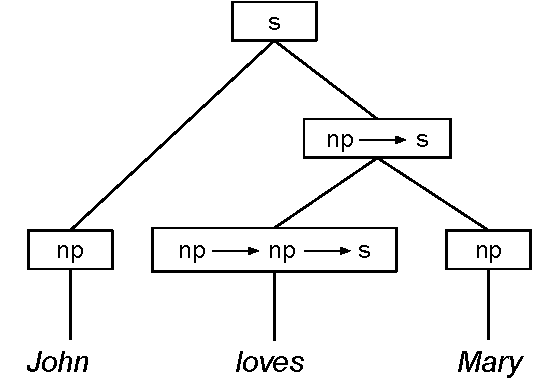
\includegraphics[width=0.4\textwidth]{images/JohnLovesMary.pdf}
\caption{Syntactic parse tree of sentence \txt{John loves Mary}.} \label{fig:JohnLovesMary}
\end{figure}

Term~\eqref{eq:ex:lovejm-2} has to be computed compositionally from lexical meanings $\I{John}$, $\I{Mary}$ and $\I{loves}$. More precisely, it has to be the result of normalizing  $\I{loves} \I{Mary} \I{John}$, as can be seen from the syntactic tree in Figure~\ref{fig:JohnLovesMary}. 

A noun phrase in Montague semantics is a term taking a static property with the type $(\iota \rightarrow o)$ as an argument and returning a static proposition with the type $o$. {\TDL} has dynamic propositions with type $(\gamma \rightarrow (\gamma \rightarrow o) \rightarrow o)$ in place of static propositions with type $o$.
This can be easily seen comparing~\eqref{eq:np:M:1} and~\eqref{eq:np:dG:1}, where $\Omega$ is an abbreviation for $(\gamma \rightarrow (\gamma \rightarrow o) \rightarrow o)$.
Equation~\eqref{eq:np:dG:2} shows the dynamic type of a noun phrase without abbeviating $(\gamma \rightarrow (\gamma \rightarrow o) \rightarrow o)$. It can be seen from this equation that the interpretation of a noun phrase is a function of three arguments (namely, a dynamic property, a context and a continuation) that returns a static proposition:
\begin{subequations}
\begin{align}
\I{np} =_{stat} \ & \underbrace{(\iota \rightarrow   o)}_{
\begin{smallmatrix}
\text{static}\\
\text{property}
\end{smallmatrix}} \rightarrow \underbrace{o}_{\begin{smallmatrix} 
\text{static}\\
\text{proposition}
\end{smallmatrix}} \label{eq:np:M:1} \\
\tr{\I{np}} =_{dyn} \ & \underbrace{(\iota \rightarrow  \Omega )}_{\begin{smallmatrix}
\text{dynamic}\\
\text{property}
\end{smallmatrix}} \rightarrow \underbrace{\Omega}_{
\begin{smallmatrix}
\text{dynamic}\\
\text{proposition}
\end{smallmatrix}} \label{eq:np:dG:1} \\
\tr{\I{np}} =_{dyn} \ & \underbrace{(\iota \rightarrow \gamma \rightarrow (\gamma \rightarrow o) \rightarrow o)}_{
\begin{smallmatrix}
\text{dynamic}\\
\text{property}
\end{smallmatrix}} \rightarrow \underbrace{\underbrace{\gamma}_{\text{context}} \rightarrow \underbrace{(\gamma \rightarrow o)}_{\begin{smallmatrix}
\text{conti--}\\
\text{nuation}
\end{smallmatrix}} \rightarrow \underbrace{o}_{\begin{smallmatrix}
\text{pro--}\\
\text{position}
\end{smallmatrix}}}_{\begin{smallmatrix}
\text{dynamic}\\
\text{proposition}
\end{smallmatrix}} \label{eq:np:dG:2}
\end{align}
\label{eq:np:MdG}
\end{subequations}

Having discussed the dynamic type of noun phrases, we can now analyse the interpretation of proper names. 
Consider, for example, the interpretation of \txt{Mary} shown in Equation~\eqref{eq:dG:Mary}. It has three arguments: a dynamic property $\P2$, a context $e$ and a continuation $\phi$. In the body of the term, property $\P2$ receives respectively constant $\textbf{m}$ (standing for \txt{Mary}), unchanged context $e$ and a continuation $(\lambda e'.\phi (\textbf{m}::{e'}))$ as arguments. Note that in $(\lambda e'.\phi (\textbf{m}::{e'}))$ an updated context $(\textbf{m}::{e'})$ is passed as an argument to the continuation $\phi$. Therefore, this updated context becomes available to the future of the computation with respect to $\etr{\I{Mary}}$. \todoK{Explain what tilda means.}
\begin{align}
\etr{\I{Mary}} =  \lambda \underbrace{{\P2}^{\iota \rightarrow \gamma \rightarrow (\gamma \rightarrow o) \rightarrow o}}_{\begin{smallmatrix}
\text{dynamic}\\
\text{property}
\end{smallmatrix}}. \underbrace{\lambda \underbrace{{e}^{\gamma}}_{\begin{smallmatrix}
\text{con--}\\
\text{text}
\end{smallmatrix}} \underbrace{{\phi}^{\gamma \rightarrow o}}_{\begin{smallmatrix}
\text{conti--}\\
\text{nuation}
\end{smallmatrix}}.\P2 \textbf{m} e (\lambda e'^{\gamma}. \phi ( \upii{\textbf{m}}{e'}))}_{
\begin{smallmatrix}
\text{dynamic}\\
\text{proposition}
\end{smallmatrix}}\label{eq:dG:Mary}
\end{align}

\comments{
\begin{align}
\etr{\I{Mary}} =  \overbrace{\lambda \underbrace{{\P2}^{\iota \rightarrow \gamma \rightarrow (\gamma \rightarrow o) \rightarrow o}}_{\begin{smallmatrix}
\text{dynamic}\\
\text{property}
\end{smallmatrix}}. \underbrace{\lambda \underbrace{{e}^{\gamma}}_{\begin{smallmatrix}
\text{con--}\\
\text{text}
\end{smallmatrix}} \underbrace{{\phi}^{\gamma \rightarrow o}}_{\begin{smallmatrix}
\text{conti--}\\
\text{nuation}
\end{smallmatrix}}. \overbrace{\overbrace{\overbrace{\P2 {\textbf{m}}^{\iota}}^{\begin{smallmatrix}
\gamma \rightarrow \\
(\gamma \rightarrow o) \rightarrow o
\end{smallmatrix}} e}^{(\gamma \rightarrow o) \rightarrow o} \ \ (\overbrace{\lambda e'^{\gamma}. \overbrace{\phi ( \overbrace{\upii{\textbf{m}}{e'}}^{\gamma})}^{o}}^{\gamma \rightarrow o})}^{o}}_{
\begin{smallmatrix}
\text{dynamic}\\
\text{proposition}
\end{smallmatrix}}}^{(\iota \rightarrow \gamma \rightarrow (\gamma \rightarrow o) \rightarrow o) \rightarrow \gamma \rightarrow (\gamma \rightarrow o) \rightarrow o}\label{eq:dG:Mary}
\end{align}
}


The interpretation of \txt{John} is analogous:
\begin{align}
\etr{\I{John}} = \lambda \P2. \lambda e \phi. \P2 \textbf{j} e (\lambda e' .\phi (\textbf{j}::{e'})) \label{eq:dG:John}
\end{align}

Transitive verbs are commonly interpreted in static semantics as terms that take two type-raised individuals and return a proposition. Their type is shown in~\eqref{eq:tvstat}. As discussed above, there should be two additional arguments (one standing for context and one standing for continuation) for a term to return a proposition in our dynamic framework. In other words, everywhere where a term of type $o$ occurs in Montague's interpretation, there has to be a term of type $(\gamma \rightarrow (\gamma \rightarrow o) \rightarrow o)$ in the dynamic framework. 
Therefore, dynamic interpretations of transitive verbs have type presented in~\eqref{eq:tvdyn} ($(\gamma \rightarrow (\gamma \rightarrow o) \rightarrow o)$ is abbreviated as $\Omega$).
\begin{subequations}
\begin{align}
\I{tv} =_{stat} \ & (\underbrace{(\iota \rightarrow   o)}_{
\begin{smallmatrix}
\text{static}\\
\text{property}
\end{smallmatrix}} \rightarrow \underbrace{o}_{
\begin{smallmatrix}
\text{static}\\
\text{propo--}\\
\text{sition}
\end{smallmatrix}}) \rightarrow (\underbrace{(\iota \rightarrow   o)}_{
\begin{smallmatrix}
\text{static}\\
\text{property}
\end{smallmatrix}} \rightarrow \underbrace{o}_{
\begin{smallmatrix}
\text{static}\\
\text{propo--}\\
\text{sition}
\end{smallmatrix}})  \rightarrow \underbrace{o}_{
\begin{smallmatrix}
\text{static}\\
\text{propo--}\\
\text{sition}
\end{smallmatrix}} \label{eq:tvstat} \\
\tr{\I{tv}} =_{dyn} \ &  (\underbrace{(\iota \rightarrow   \Omega)}_{
\begin{smallmatrix}
\text{dynamic}\\
\text{property}
\end{smallmatrix}} \rightarrow \underbrace{\Omega}_{
\begin{smallmatrix}
\text{dynamic}\\
\text{propo--}\\
\text{sition}
\end{smallmatrix}}) \rightarrow (\underbrace{(\iota \rightarrow   \Omega)}_{
\begin{smallmatrix}
\text{dynamic}\\
\text{property}
\end{smallmatrix}} \rightarrow \underbrace{\Omega}_{
\begin{smallmatrix}
\text{dynamic}\\
\text{propo--}\\
\text{sition}
\end{smallmatrix}})  \rightarrow \underbrace{\Omega}_{
\begin{smallmatrix}
\text{dynamic}\\
\text{propo--}\\
\text{sition}
\end{smallmatrix}}  \label{eq:tvdyn}
\end{align} \label{eq:tv:MdG}
\end{subequations}

Then the subject wide scope interpretation $\tr{\I{loves}}$ of \txt{loves} is as follows:
\begin{flalign}
\phantom{a} & \lambda \Y2^{(\iota \rightarrow \Omega) \rightarrow \Omega} \X2^{(\iota \rightarrow \Omega) \rightarrow \Omega}. \X2 ( \lambda \x1^{\iota}. \Y2 (\lambda \y1^{\iota}. (  \lambda {e}^{\gamma} \phi^{\gamma \rightarrow o}. {\textbf{love}}^{\iota \rightarrow \iota \rightarrow o} {\x1} {\y1} \land \phi e) ) ) &  \label{eq:dG:love} 
\end{flalign}

Note that the dynamic interpretation~\eqref{eq:dG:love} is analogous to the static interpretation of the verb. Indeed, compare~\eqref{eq:lovedyn} showing dynamic $\tr{\I{loves}}$ and~\eqref{eq:lovestat} showing static  $\I{loves}$:
\begin{align}
\I{loves} = \  & \lambda \Y1 \X1. \X1( \lambda \x1. \Y1 (\lambda \y1. \textbf{love} \x1 \y1 ))  \label{eq:lovestat} \\
\tr{\I{loves}} = \ & \lambda \Y2 \X2. \X2( \lambda \x1. \Y2 (\lambda \y1. ( \lambda e \phi. \textbf{love} \x1 \y1 \land \phi e )))  \label{eq:lovedyn}
\end{align}
The terms are stucturally similar. The only deviation in structure is the subterm  $( \lambda e \phi. \textbf{love} \x1 \y1 \land \phi e )$ in~\eqref{eq:lovedyn} in place of $\textbf{love} \x1 \y1$ in~\eqref{eq:lovestat}. This deviation is explained by the fact that all static propositions, i.e. terms of type $o$, are translated into dynamic propositions, i.e. terms of type $(\gamma \rightarrow (\gamma \rightarrow o) \rightarrow o )$.
The subterm  $( \lambda e \phi. \textbf{love} \x1 \y1 \land \phi e )$ is such a dynamic proposition.

Now, given dynamic lexical interpretations~\eqref{eq:lovedyn},~\eqref{eq:dG:Mary} and~\eqref{eq:dG:John} of \txt{loves}, \txt{Mary} and \txt{John} respectively, the meaning~\eqref{eq:ex:lovejm-2} of Sentence~\eqref{sent:JlovesM-2006}  can be compositionally computed. Example~\ref{ex:S1} illustrates this computation.

\begin{example}[Meaning of \txt{John loves Mary}, $\S_1$]
\begin{align}
\S_1 = \ & \tr{\I{loves}} \etr{\I{Mary}} \etr{\I{John}}  \notag \\
= \ & (\lambda \Y2 \X2. \X2( \lambda \x1. \Y2 (\lambda \y1. ( \lambda e' \phi. \textbf{love} \x1 \y1 \land \phi e' ))) )  \etr{\I{Mary}} \etr{\I{John}}  \notag \\
\bconv \ & (\lambda  \X2. \X2( \lambda \x1. \I{Mary}  (\lambda \y1. ( \lambda e' \phi. \textbf{love} \x1 \y1 \land \phi e' ))) )  \etr{\I{John}}  \notag \\
\bconv \ &   \etr{\I{John}}( \lambda \x1. \I{Mary}  (\lambda \y1. ( \lambda e' \phi. \textbf{love} \x1 \y1 \land \phi e' )))   \notag \\
= \ &   \etr{\I{John}}( \lambda \x1. (\lambda \P2. \lambda e \phi. \P2 \textbf{m} e (\lambda e. \phi (\upii{\textbf{m}}{e'})))  (\lambda \y1. ( \lambda e' \phi. \textbf{love} \x1 \y1 \land \phi e' )))   \notag \\
\bconv \ &    \etr{\I{John}}( \lambda \x1.  \lambda e \phi. (\lambda \y1. ( \lambda e' \phi. \textbf{love} \x1 \y1 \land \phi e' )) \textbf{m} e (\lambda e'. \phi (\upii{\textbf{m}}{e'})))   \notag \\
\bconv \ &   \etr{\I{John}}( \lambda \x1.  \lambda e \phi. ( \lambda e' \phi. \textbf{love} \x1 \textbf{m} \land \phi e' ) e (\lambda e' . \phi (\upii{\textbf{m}}{e'})))   \notag \\
\bred \ & \etr{\I{John}}( \lambda \x1.  \lambda e \phi.  \textbf{love} \x1 \textbf{m} \land  (\lambda e' .\phi (\upii{\textbf{m}}{e'}) e))   \notag \\
\bconv \ &  \etr{\I{John}}( \lambda \x1.  \lambda e \phi.  \textbf{love} \x1 \textbf{m} \land  \phi (\upii{\textbf{m}}{e} ))   \notag \\
= \ &    ( \lambda \P2. \lambda e \phi. \P2 \textbf{j} e (\lambda e' .\phi (\upii{\textbf{j}}{e'})))( \lambda \x1.  \lambda e \phi.  \textbf{love} \x1 \textbf{m} \land  \phi (\upii{\textbf{m}}{e} ))   \notag \\
\bconv \ &    \lambda e \phi. ( \lambda \x1.  \lambda e \phi.  \textbf{love} \x1 \textbf{m} \land  \phi (\upii{\textbf{m}}{e} ))   \textbf{j} e (\lambda e' . \phi (\upii{\textbf{j}}{e'})) \notag \\
\bred \ &    \lambda e \phi.  \textbf{love}  \textbf{j} \textbf{m} \land   (\lambda e' .\phi (\upii{\textbf{j}}{e'})) (\upii{\textbf{m}}{e} )  \notag \\
\bconv \ &    \lambda e \phi.  \textbf{love}  \textbf{j} \textbf{m} \land   \phi (\upii{\textbf{j}}{\upii{\textbf{m}}{e} })  \label{eq:2006:JohnLovesMary} 
\end{align} \label{ex:S1} \qex
\end{example}

We have analyzed how, using continuation technique, a context can be made available in the following computation. For example, in the subterm $\phi (\textbf{j}::\textbf{m}::e)$ of the computed dynamic interpretation~\eqref{eq:2006:JohnLovesMary} constants $\textbf{m}$ for \txt{Mary} and $\textbf{j}$ for \txt{John} are provided for the future of the computation of the meaning of whole discourse from the perspective of the interpretation $\S_1$. 
These constants should be \emph{accessed} when necessary. 

A common task when accessing a context is the choice of an anaphoric reference. For this, we define a special function $\selK$ of type $(\gamma \rightarrow \iota)$ that takes a context as an argument and returns an individual. The mechanism of anaphora resolution is to be implemented within $\selK$. For the sake of simplicity and for keeping focus on developing the core of \TDL, we avoid the implementation of any particular anaphora resolution algorithm\footnote{The avoidance of anaphora resolution implementation is also motivated by our desire to emphasise that the framework is not restricted by any particular anaphora resolution algorithm. In contrast, it is flexible to incorporate any desirable algorithm within $\selK$. This is particularly relevant, as the research in anaphora resolution is steadily evolving.} in this paper and assume that $\selK$ always returns a correct individual from a given context. 

Function $\selK$ allows us to interpret pronouns, as illustrated for the pronoun \txt{he} in~\eqref{eq:he:2006}:
\begin{align}
\etr{\I{he}} =  \lambda \P2^{\iota \rightarrow \gamma \rightarrow (\gamma \rightarrow o) \rightarrow o}. \lambda e^{\gamma} \phi^{\gamma \rightarrow o}. \P2 ( \selK_{he} e ) e \phi  \label{eq:he:2006}
%\I{he} = \lambda \P2. \lambda e \phi. \P2 (\selK_{he}e)e\phi
\end{align}
Compare interpretation $\etr{\I{he}}$~\eqref{eq:he:2006} and interpretation $\etr{\I{Mary}}$~\eqref{eq:dG:Mary}. They differ in two respects. Firstly, while the dynamic property $\P2$ is applied to a specific individual which is the constant $\textbf{m}$ in $\etr{\I{Mary}}$, it is applied to $( \selK_{he} e )$ in $\etr{\I{he}}$. It is the responsibility of the selection function to return the required individual. Secondly, while the third argument of $\P2$ in $\etr{\I{Mary}}$ is the continuation containing context updated with $\textbf{m}$, no context update happens in $\etr{\I{he}}$.

\begin{figure}[h]
 \centering
    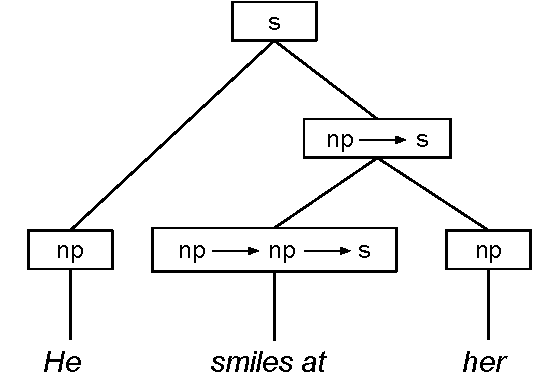
\includegraphics[width=0.4\textwidth]{images/HeSmilesatHer.pdf}
\caption{Syntactic parse tree of sentence \txt{He smiles at her}.} \label{fig:ptS3-2006}
\end{figure}

Having defined dynamic interpretations of pronouns, we can now compute the dynamic meaning of the sentence~\eqref{HeSmilesAtHer-2006}. Its parse-tree is presented in Figure~\ref{fig:ptS3-2006}.
\enumsentence{\txt{He smiles at her.} \label{HeSmilesAtHer-2006}}


\begin{example}[Meaning of \txt{He smiles at her}, $\S_2$] \label{ex:2006:HeSmilesAtHer} 
\begin{align}
\S_2 = \ & \tr{\I{smiles\_at}} \etr{\I{her}} \etr{\I{he}} \notag \\
 = \ & (\lambda \Y2 \X2. \X2( \lambda \x1. \Y2 (\lambda \y1. ( \lambda e' \phi. \textbf{smile} \x1 \y1 \land \phi e' ))) )  \etr{\I{her}} \etr{\I{he}} \notag \\
\bconv \ & (\lambda  \X2. \X2( \lambda \x1.  \etr{\I{her}}  (\lambda \y1. ( \lambda e' \phi. \textbf{smile} \x1 \y1 \land \phi e' ))) ) \etr{\I{he}} \notag \\
\bconv \ &   \etr{\I{he}}  ( \lambda \x1.  \etr{\I{her}}  (\lambda \y1. ( \lambda e' \phi. \textbf{smile} \x1 \y1 \land \phi e' ))) \notag  \\
= \ &   \etr{\I{he}} ( \lambda \x1.  (\lambda \P2. \lambda e \phi. \P2 (\selK_{her}e)e\phi)  (\lambda \y1. ( \lambda e' \phi. \textbf{smile} \x1 \y1 \land \phi e' ))) \notag \\
 \bconv \ &  \etr{\I{he}}  ( \lambda \x1.  (\lambda e \phi.  (\lambda \y1. ( \lambda e' \phi. \textbf{smile} \x1 \y1 \land \phi e' )) (\selK_{her}e)e\phi) ) \notag \\
  \bconv \ &  \etr{\I{he}}  ( \lambda \x1.  (\lambda e \phi.   ( \lambda e' \phi. \textbf{smile} \x1  (\selK_{her}e) \land \phi e' ) e\phi) ) \notag \\
 \bred \ &   \etr{\I{he}}  ( \lambda \x1.  (\lambda e \phi.  \textbf{smile} \x1  (\selK_{her}e) \land \phi e) ) \notag \\
  = \ &  (\lambda \P2. \lambda e \phi. \P2 (\selK_{he}e)e\phi) ( \lambda \x1.  (\lambda e \phi.  \textbf{smile} \x1  (\selK_{her}e) \land \phi e) ) \notag \\
\bconv \ & \lambda e \phi. ( \lambda \x1.  (\lambda e \phi.  \textbf{smile} \x1  (\selK_{her}e) \land \phi e) )  (\selK_{he}e)e\phi \notag \\
\bconv \ & \lambda e \phi.   (\lambda e \phi.  \textbf{smile}  (\selK_{he}e)  (\selK_{her}e) \land \phi e) e\phi \notag \\
\bred \ & \lambda e \phi.   \textbf{smile}  (\selK_{he}e)  (\selK_{her}e) \land \phi e \label{eq:2006:HeSmilesAtHer}
\end{align} \qex
\end{example}


Sentence~\eqref{HeSmilesAtHer-2006} is meaningful in the sense that it has interpretation~\eqref{eq:2006:HeSmilesAtHer}. However, when the sentence is isolated, anaphora cannot be resolved. Function $\selK$ can return individuals for \txt{he} and \txt{her} only when the sentence is evaluated over some context containing the corresponding antecedents. This happens when the sentence is uttered in a certain discourse. 

Following the principle of compositionality, the meaning of a discourse is computed compositionaly from from the meanings of its sentences. Since a discourse is a sequence of sentences, we perform the computation of its meaning incrementally, starting from the first sentence in the order as the sentences appear. We say that each new sentence \emph{updates} the meaning of the current discourse. The pronominal anaphora can then be resolved during this discourse update. 

To define the discourse update function we shall decide the type of discourse meaning. Recall the type $( \gamma \rightarrow (\gamma \rightarrow o) \rightarrow o )$ of sentence meaning first. Informally, one can think of the meaning of an individual sentence as something that has to be evaluated with respect to a context to be fully understood.  A discourse, on the other hand, can be seen as something that already has a concrete context. Therefore, interpretations of discourses can be defined as the terms of type~\eqref{eq:typediscourse}:
\begin{align}
\I{d} =  (\gamma \rightarrow o) \rightarrow o \label{eq:typediscourse}
\end{align}
Thus, we represent the meaning of the current discourse as a term that takes a continuation as its only argument. The continuation is necessary for the computation of the meaning of the remainder of the discourse.  


Now the discourse update function $\updt$ can be defined. This function takes two arguments, namely, the meaning of the current discourse and the meaning of the new sentence.
\begin{definition}[Discourse update] Let $\D$ be a term of type $( (\gamma \rightarrow o) \rightarrow o)$ and $\S$ be a term of type $(\gamma \rightarrow (\gamma \rightarrow o) \rightarrow o)$. Then the function $ \updt$ is defined by the following equation:
\begin{align} %\label{eq:DisUpd-simple} 
 \updt \ \D \ \S \defeq  \lambda \phi.   \D (\lambda e. \S e \phi) \label{eq:updt}
\end{align} \label{def:updt-prelim}
\end{definition}
The update of the interpretation $\D$ of the current discourse with the interpretation $\S$ of a new sentence results in the interpretation of the discourse containing the new sentence (as its last sentence). Therefore, the resulting term has to be of type $((\gamma \rightarrow o) \rightarrow o)$. Hence, the term should have only one argument of type $(\gamma \rightarrow o)$. This explains the abstraction over the variable $\phi$ in~\eqref{eq:updt}. The body of the term must be a term of type $o$ contributed by $\D$ and $\S$. $\D$ should go first in the logical formula. It requires one argument of type $(\gamma \rightarrow o)$, which should be constructed with $\S$ of type $(\gamma \rightarrow (\gamma \rightarrow o) \rightarrow o)$. This explains the subterm $(\lambda e. \S e \phi) $. Importantly, $(\lambda e. \S e \phi) $ functions as a continuation of $\D$. Therefore, the context of $\D$ is available for $\S$ (and $\S$ can update the context!). Indeed, the context of $\D$ is passed as the first argument of $\S$ due to the fact that the subterm $(\lambda e. \S e \phi) $ is an abstraction.

We consider that the very first sentence is always uttered in a context-empty discourse interpreted in the following way:
\begin{definition}[Interpretation of initial content-empty discourse] Let $c$ be a context. Then the initial (content-empty) discourse containing context $c$ is interpreted as the following term:
\begin{align}
\D_0 \defeq \lambda \phi. \phi c \label{eq:D0}
\end{align}
\end{definition}

A realistic context $c$ should contain common knowledge and information learned since an agent interpreting the discourse was put into functioning. For simplification, however, context $c$ in the initial discourse can be considered either empty or containing only a necessary part of some knowledge. By letting context be a list of individuals (i.e. by letting $\gamma$ be $\texttt{ list of } [  \iota  ]$), the empty context can be represented by the empty list~$\nil$.

Now we can compute the meaning of discourse~\eqref{sent:JlovesMHesmilesatHer}, given the meanings $\S_1$~\eqref{ex:S1} and $\S_2$~\eqref{eq:2006:HeSmilesAtHer} of the sentences composing it. Example~\eqref{ex:D2} illustrates this computation.
\enumsentence{ \txt{John loves Mary. He smiles at her.} \label{sent:JlovesMHesmilesatHer}}

\begin{example}[Meaning of \txt{John loves Mary. He smiles at her.}, $\D_2$]
\begin{align}
\D_1 = \ & \updt \ \D_0 \ \S_1 \notag \\
= \ &  \lambda \phi.   \D_0 (\lambda e. \S_1 e \phi)  \tag{by~\eqref{eq:updt}} \\
= \ & \lambda \phi.   (\lambda \phi. \phi \ \nil)  (\lambda e. \S_1 e \phi) \tag{by~\eqref{eq:D0}} \\
\bconv \ & \lambda \phi.    (\lambda e. \S_1 e \phi) \  \nil  \notag \\
\bconv \ & \lambda \phi.    \S_1 \ \nil \ \phi  \notag \\
= \ & \lambda \phi.    ( \lambda e \phi.  \textbf{love}  \textbf{j} \textbf{m} \land   \phi (\upii{\textbf{j}}{\upii{\textbf{m}}{e} })) \ \nil \ \phi  \tag{by~~\eqref{sent:JlovesMHesmilesatHer}} \\
\bred  \ & \lambda \phi.    \textbf{love}  \textbf{j} \textbf{m} \land   \phi (\textbf{j} :: \textbf{m}::\nil)  \label{eq:D1} 
\end{align}
\begin{flalign}
\D_2 = \ & \updt \ \D_1 \ \S_2 & \notag \\
= \ &  \lambda \phi.   \D_1 (\lambda e. \S_2 e \phi)  & \tag{by~\eqref{eq:updt}} \\
= \ &  \lambda \phi.   \D_1  (\lambda e. (\lambda e \phi.   \textbf{smile}  (\selK_{he}e)  (\selK_{her}e) \land \phi e ) e \phi) & \tag{by~\eqref{eq:2006:HeSmilesAtHer}} \\
\bred \ &  \lambda \phi.   \D_1  (\lambda e.    \textbf{smile}  (\selK_{he}e)  (\selK_{her}e) \land \phi e ) & \notag \\
= \ &  \lambda \phi.   ( \lambda \phi.    \textbf{love}  \textbf{j} \textbf{m} \land   \phi (\textbf{j} :: \textbf{m}::\nil)) (\lambda e.    \textbf{smile}  (\selK_{he}e)  (\selK_{her}e) \land \phi e )  & \tag{by~\eqref{eq:D1}} \\
\bconv \ &  \lambda \phi.       \textbf{love}  \textbf{j} \textbf{m} \land   (\lambda e.    \textbf{smile}  (\selK_{he}e)  (\selK_{her}e) \land \phi e )   (\textbf{j} :: \textbf{m}::\nil) & \notag \\
\bred \ &  \lambda \phi.       \textbf{love}  \textbf{j} \textbf{m} \land     \textbf{smile}  (\selK_{he} (\textbf{j} :: \textbf{m}::\nil))  (\selK_{her} (\textbf{j} :: \textbf{m}::\nil)) \land \phi  (\textbf{j} :: \textbf{m}::\nil) & \label{eq:D2}  
\end{flalign}
 \label{ex:D2}
\end{example}

%Interpretation~\eqref{eq:D2} of discourse~\eqref{sent:JlovesMHesmilesatHer} was obtained in a truly compositional fashion. 

Observe that during the computation of $\D_2$, the context $(\textbf{j} :: \textbf{m}::\nil)$ coming from the interpretation $\S_1$ of the first sentence was passed via $\beta$-reduction to $\selK$ operators coming from interpretation $\S_2$ of the second sentence. In other words, $\selK$ operators compositionally obtained access to the context $(\textbf{j} :: \textbf{m}::\nil)$. Having an anaphora resolution algorithm implemented, $\selK$ would select appropriate individuals from $(\textbf{j} :: \textbf{m}::\nil)$. Then
the following semantic representation of~\eqref{sent:JlovesMHesmilesatHer} would be obtained: 
\begin{align}
\lambda \phi.\textbf{love} \  \textbf{j} \ \textbf{m} \land    \textbf{smile}  \ \textbf{j} \ \textbf{m} \land \phi   (\textbf{j} :: \textbf{m}::\nil) \label{int:JLMHeSH:2006-2}
\end{align}


Since the context $ (\textbf{j} :: \textbf{m}::\nil)$ in~\eqref{int:JLMHeSH:2006-2} is the argument of the continuation $\phi$ of the discourse, it is accessible for future computation. This means that the individuals $\textbf{j}$ and $\textbf{m}$ can continue to serve as ancestors for anaphoric pronouns in the following sentences. 
